\subsection{Frozen-method training replication}\label{app:seed-replication}
We repeat the initial physical-head-only models; their later geometric refinement is reported in Appendix~\ref{app:geometric-recovery}. Architecture, final-checkpoint schedules, strength four, and hydrogen-flow settings are fixed before the new fits. Each FM parent receives 15,000 two-pass updates at batch size 32, and GAGA receives 30,000 one-pass updates. Within a pair, initialization tensors and the batch-schedule prefix match. Backbone example-forward counts match, while optimizer steps, data presentations, and runtime differ. Every model uses its prescribed final checkpoint.

The new metadata pool excludes all compositions from the previous pool. Only 20 previously unused 17--28-atom compositions pass qualification, rather than the planned 32. We therefore select these 20 and the first 44 eligible 29--40-atom compositions by the fixed metadata ranking before generation. The original selection plan and qualification results are archived. All 64 compositions are absent from the processed generator corpora and prepared training/validation rows. Eligibility uses reference geometry and overlap checks, not generated outcomes or energies.

Strength-zero and strength-four trajectories share source draws and sampler randomness. Recorded zero-strength budgets include head calls multiplied by zero. Each corrected structure is evaluated unchanged, after the fixed radial readout, and after the learned hydrogen readout. The hydrogen readout leaves graph-valid parent outputs unchanged. Identical coordinates reuse their physical calculation; failures remain in rate denominators.

The three new pairs form the primary independent-training analysis. A separate five-pair summary includes the two development fits. Composition intervals resample the 64 compositions conditional on fitted models; crossed intervals also resample fit indices. Equal-weight size-stratum averages supplement the pooled 20:44 mixture. Training-variation estimates are based on only three new or five total fits.

\begin{table}[htbp]\centering\small\caption{Joint yield in every fit (percent). Fits 1--2 reuse earlier weights; fits 3--5 are newly trained.}\begin{tabular}{llrrrrr}\toprule Parent & Module & 1 & 2 & 3 & 4 & 5\\\midrule
FM & None & 9.96 & 7.52 & 3.61 & 6.25 & 8.69\\
FM & Physical & 28.22 & 26.37 & 11.72 & 24.71 & 29.00\\
FM & Physical + radial & 30.18 & 27.83 & 12.70 & 27.15 & 32.42\\
FM & Physical + H flow & 30.66 & 28.03 & 12.89 & 27.34 & 32.71\\
GAGA & None & 12.30 & 6.64 & 11.52 & 8.59 & 4.69\\
GAGA & Physical & 27.34 & 24.02 & 28.61 & 27.34 & 19.53\\
GAGA & Physical + radial & 27.93 & 24.22 & 29.20 & 27.83 & 19.73\\
GAGA & Physical + H flow & 27.93 & 24.22 & 29.00 & 27.83 & 19.73\\
\bottomrule\end{tabular}\end{table}

\begin{figure}[htbp]\centering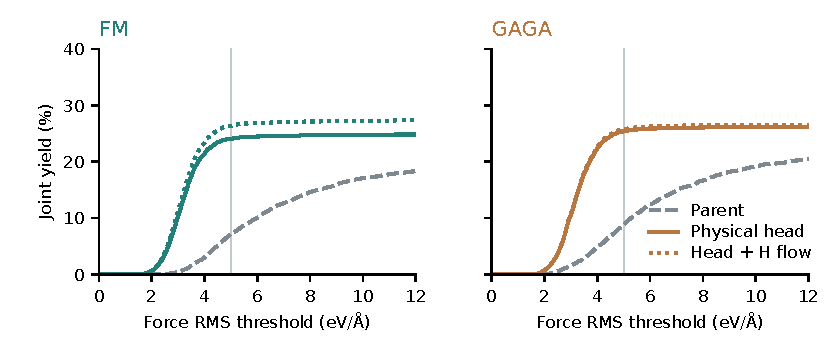
\includegraphics[width=\linewidth]{../research/figures/final_complete_v1/figures/force_thresholds.pdf}\caption{Joint yield versus force threshold, averaged over all five fits. The vertical line marks the prespecified 5 eV/\AA\ criterion; the curves do not select a new threshold.}\end{figure}

For FM, physical correction adds 16.80 pooled joint-yield points (crossed interval $[11.50,21.93]$) and 19.34 equal-stratum points ($[13.85,24.69]$). GAGA gains 16.62 pooled points ($[12.95,20.47]$) and 18.46 equal-stratum points ($[14.32,22.72]$). After hydrogen readout, FM minus GAGA is 0.59 pooled points ($[-8.59,8.59]$) and 0.95 equal-stratum points ($[-8.93,9.63]$).

The study adds 20,480 evaluation parent trajectories, 20,480 derived readout outputs, and 22,688 GFN2 attempts. New teachers use 1,536 training trajectories and 6,144 eSEN queries. The three new pairs add 135,000 parent, 120,000 head, and 30,000 hydrogen-model updates. Reused calculations are counted only once.

Six GFN2 calculations initially fail electronic convergence, all on graph-invalid coordinates. Increasing the SCC limit from 250 to 1,000 resolves all six while preserving coordinates, charge, spin, electronic temperature, Hamiltonian, and accuracy. Original failures are archived; completion changes no graph or joint count. All-output energy analyses use the completed scores. Of 1,384 FM pairs valid under both hydrogen readouts, 111 are newly repaired under both. On this descriptive subset, the learned readout lowers energy by 83.42 meV/atom relative to the radial rule.
